En este capítulo se expondrán las distintas tecnologías usadas para el desarrollo del proyecto así como el repositorio en GitHub donde se encuentra almacenado el código fuente del proyecto.

\newpage

\section{Base de Datos}
Aquí expondremos el tipo de base de datos utilizado, así los métodos usados para desplegarlo tanto en local como en remoto.

\subsection{PostgreSQL}
La base de datos que se ha utilizado para este proyecto es PostgreSQL \cite{postgresql}. Hemos elegido este Sistema Gestor de Base de Datos (SGBD) debido a su gran versátilidad y debido a que continene una cantidad de caracteristicas que otras base de datos como MySQL \cite{mysql} o MariaDB \cite{mariadb} no tienen.

Además, su integración con el ORM (Object Relational Mapping) Sequelize \cite{sequelize} es prácticamente total, dando Sequelize soporte casi a la mayoría de las caracteristicas que te permite el SGBD PostgreSQL.

\subsection{Docker}
Para desplegar la base de datos, hemos usado una imagen Docker, para así evitar usar una instalación en local con una versión en concreto y arriesgarnos que con futuras actualizaciones de los sistemas operativos subyacentes den problemas.

A continuación, exponemos el código del docker-compose.yml en el Listado 6.1.

\begin{lstlisting}[language=XML,caption={docker-compose.yml},captionpos=b]
version: '3'
services:
  postgresql:
    image: postgres:9.6
    volumes:
      - smartrural:/var/lib/postgresql/data
    ports:
      - 5432:5432
    environment:
      - POSTGRES_DB=smartrural
      - POSTGRES_USER=smartrural
      - POSTGRES_PASSWORD=smartrural
volumes:
  smartrural:
    external: false
\end{lstlisting}

\subsection{Relational Database Service}
Por último, respecto a la base de datos, para tener una base de datos remota que pueda usar el software cuando se instala en el dominio remoto, hemos usado el servicio de Amazon Web Services (AWS) llamado Relational Database Service (RDS).

Debido a cuestiones económicas, hemos decidido optar por esta implementación de AWS en vez de usar la base de datos de Azure. Así que, al ser este un sistema puramente distribuido, da igual donde se aloje la base de datos. Mientras que se pueda acceder a ella de forma pública con una conexión de internet, es un servicio perfectamente válido.

A continuación, en la Figura 6.1 se puede apreciar la base de datos en el portal web de AWS.

\begin{figure}[H]
    \centering
    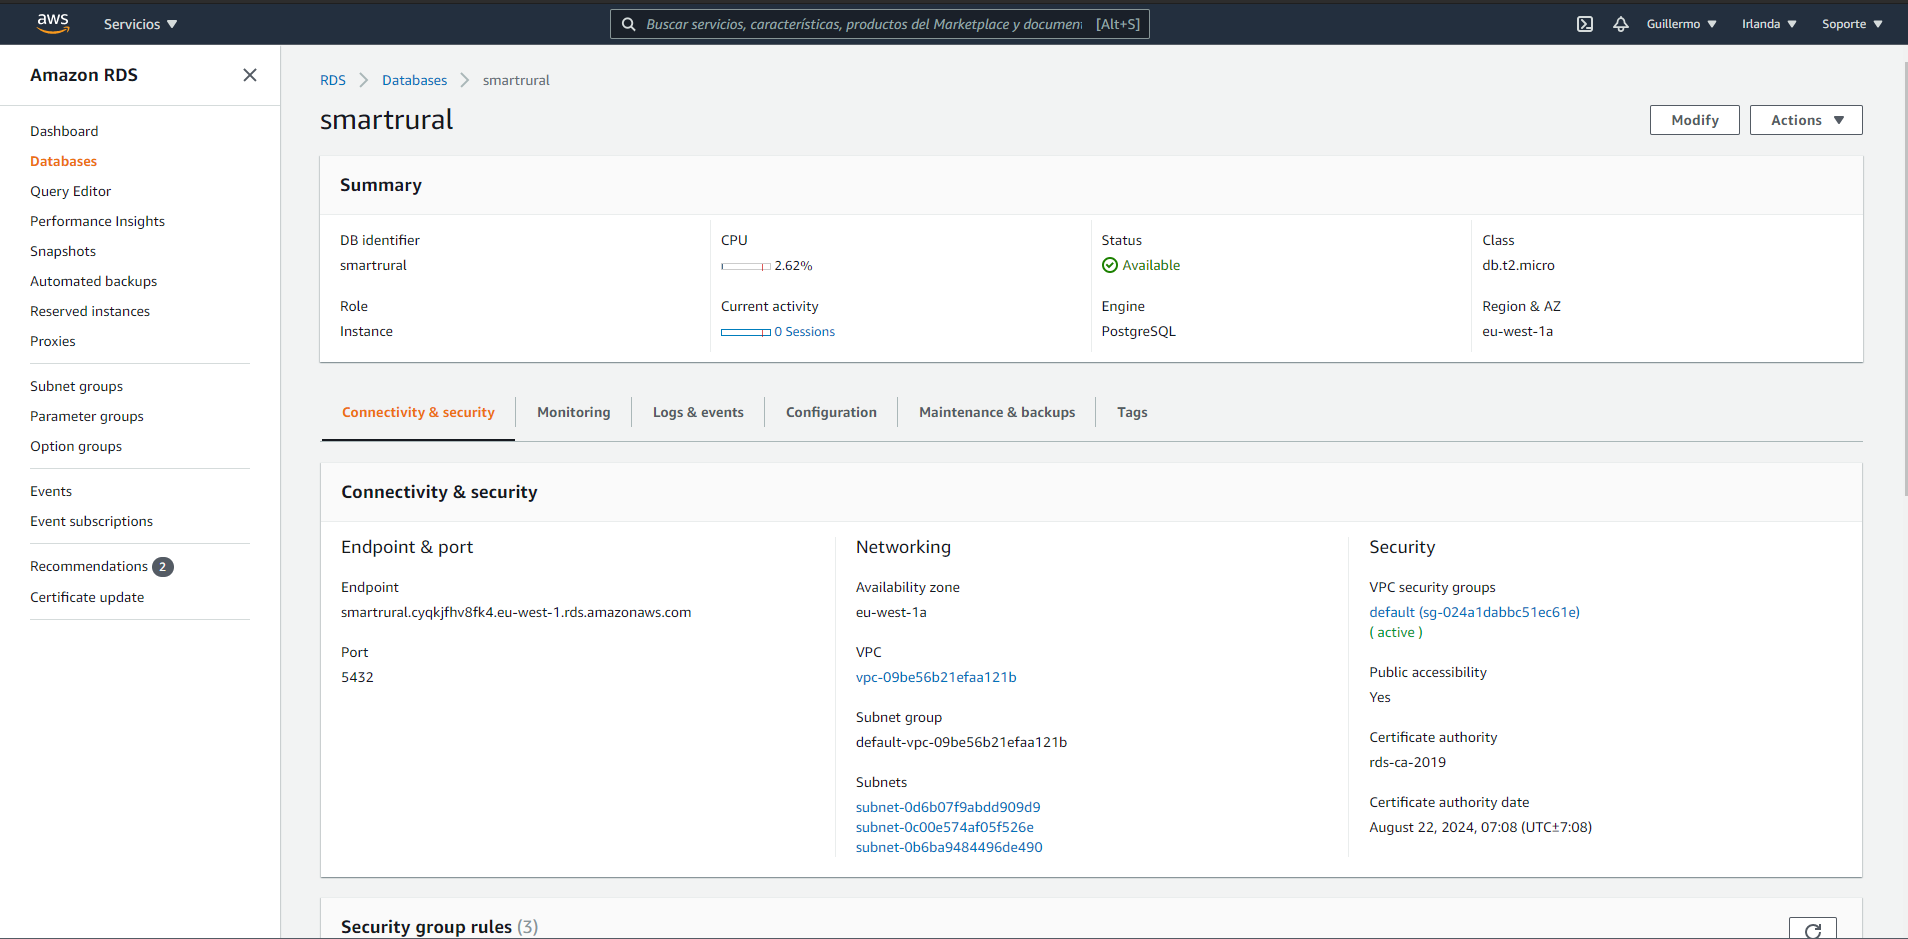
\includegraphics[width=1\linewidth]{images/implementation/database/aws rds.png}
    \caption{AWS RDS PostgreSQL}
\end{figure}

\section{Backend}
Aquí expondremos las distintas partes que conforman el backend y como se relacionan entre sí.

\subsection{Modelo de datos}
Para facilitar el uso de la base de datos y hacer un Create Read Update Delete (CRUD) en sus tablas, se ha usado un ORM y el concepto de modelo de datos, para crear entidades vivientes en lugar de operaciones sobre tablas de base de datos.

Los modelos usados son:

\begin{itemize}
    \item Auth: modelo usado para almacenar el token de sesión del login del usuario.
    \item Crop: modelo usado para almacenar los cultivos.
    \item CropPhytosanitary: modelo usado para relacionar un cultivo con un fitosanitario.
    \item Event: modelo usado para almacenar los eventos complejos a los que suscribirse.
    \item FarmableLand: modelo para almacenar los terrenos de un usuario.
    \item FarmableLandCrop: modelo para relacionar los terrrenos con un cultivo.
    \item FirebaseToken: modelo para almacenar los token de las notificaciones push de un usuario.
    \item Irrigate: modelo para almacenar los riegos de un terreno.
    \item Notification: modelo para almacenar las notificaciones de un usuario.
    \item Phytosanitary: modelo para almacenar los fitosanitarios.
    \item User: modelo para almacenar los usuarios.
    \item UserEvent: modelo para relacionar a un usuario con una serie de eventos complejos.
    \item UserSensor: modelo para relacionar a una serie de sensores con un usuario.
    \item UserSettings: modelo para almacenar los ajustes del sistema de un usuario.
\end{itemize}

Estos modelos han sido declarados todos en archivos con formato de tipo JavaScript (JS).

A continuación, exponemos en la Figura 6.2 la ruta de donde se declaran los modelos y en el Listado 6.2 la declaración de un modelo en código fuente.

\begin{figure}[H]
    \centering
    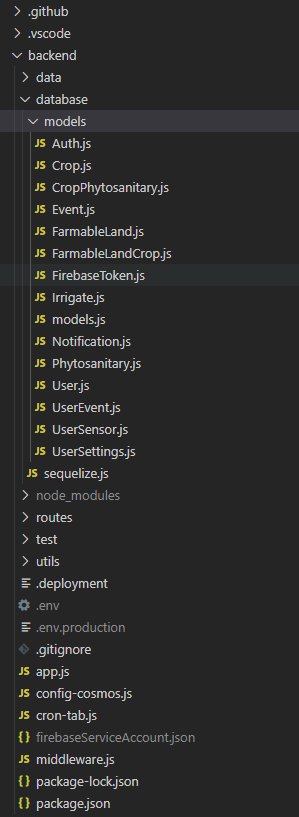
\includegraphics[width=0.4\linewidth]{images/implementation/backend/backend models.png}
    \caption{Estructura del Backend con los modelos}
\end{figure}

\begin{lstlisting}[language=Java,caption={Declaración de modelo},captionpos=b]
const { Model, DataTypes } = require('sequelize');

const sequelize = require('../sequelize');
const User = require('./User');

class Auth extends Model {}

Auth.init({
  id: {
    type: DataTypes.BIGINT,
    autoIncrement: true,
    primaryKey: true
  },
  jwt: {
    type: DataTypes.STRING
  },
  expires: {
    type: DataTypes.DATE
  }
}, {
  sequelize,
  modelName: 'Auth',
  freezeTableName: true,
  tableName: 'Auth',
  timestamps: true,
});

Auth.prototype.isValid = function() {
  return (
    new Date(this.expires).getTime() >= new Date().getTime()
  );
}

Auth.belongsTo(User);

module.exports = Auth;
\end{lstlisting}

\subsection{Sequelize}
Para trasladar los modelos anteriormente descritos a tablas de base de datos con sus columnas y demás propiedades, se ha usado el ORM Sequelize. Este ORM es sumamente versátil y muy completo, y en caso de que el día de mañana se quisiera cambiar de SGBD, solo tendríamos que cambiar el tipo del dialecto a usar.

Así pues, tan solo con un reinicio del Backend, podriamos pasar de usar una base de datos en PostgreSQL a una en MySQL, SQL Server, SQLite o cualquier otra típico SGBD del mercado.

A continuación, en el Listado 6.3 se muestra como se instancia Sequelize con los valores predeterminados.

\begin{lstlisting}[language=Java,caption={Creación de instancia de Sequelize},captionpos=b]
const { Sequelize } = require('sequelize');

let dialectOptions = {};
if(process.env.ENVIRONMENT === 'production')
{
  dialectOptions = {
    ssl: {
      require: true,
      rejectUnauthorized: false
    }
  }
}

const sequelize = new Sequelize(
  process.env.DATABASE_NAME,
  process.env.DATABASE_USERNAME,
  process.env.DATABASE_PASSWORD,
  {
    host: process.env.DATABASE_HOST,
    dialect: process.env.DATABASE_DIALECT,
    dialectOptions: dialectOptions,
    logging: (process.env.ENVIRONMENT === 'production'),
  }
);

module.exports = sequelize;
\end{lstlisting}

\subsection{Servicios}
Para mejorar la modularización de todo el backend y que de forma efectiva se pueda cambiar la lógica cuando se necesite, hemos creado una capa de servicios.

Dichos servicios son llamados desde de los controladores y desde de los servicios de creación de base de datos con datos de ejemplo.

Además, estos servicios también son usados en los test, por lo cual, si más adelante se cambia la lógica de los servicios, mientras se mantenga la precondición y la postcondición, los test seguirán funcionando.

A continuación, en el Listado 6.4, exponemos el servicio de envio de creación de usuarios como ejemplo de servicio.

\begin{lstlisting}[language=Java,caption={Servicio de Creación de Usuario},captionpos=b]
const User = require('../../database/models/User');
const { setPassword } = require('../../utils/password');

const createUser = async(username, password, fullname) => {
  const { hash, salt } = setPassword(password);
  return await User.create({
    username: username,
    password: hash,
    salt: salt,
    fullname: fullname,
    isActive: true
  });
};

module.exports = {
  createUser
};
\end{lstlisting}

\subsection{Middleware}
Uno de los aspectos más importantes para nuestro backend es la seguridad. Y para ello, tenemos que establecer un sistema de login seguro, fiable y fácilmente resoluble.

Este sistema de login, se comprueba mediante este middleware. Cada vez que se accede a un endpoint distinto al de login, se comprueba que el token de sesión existe y es veraz. Si no lo es, al pasar por ese middleware, el endpoint automáticamente dara un error con el código 401 Unauthorized.

A continuación, exponemos en el Listado 6.5 la codificación del middleware que se usa en la totalidad de los endpoints \cite{endpoint}.

\begin{lstlisting}[language=Java,caption={Middleware},captionpos=b]
const Auth = require('./database/models/Auth');
const User = require('./database/models/User');
const { Op } = require('sequelize');
const { verifyToken } = require('./utils/jwt');

const middleware = async (req, res, next) => {
  try
  {
    const token = (req.headers['authorization'] !== null) ? req.headers['authorization'].split(' ')[1] : null;
    if (token)
    {
      const auth = await Auth.findOne({
        where: {
          jwt: token,
          expires: {
            [Op.gt]: new Date()
          }
        }
      });

      if(auth && auth.isValid())
      {
        const user = await User.findOne({
          where: {
            id: auth.UserId
          }
        });
        const verify = verifyToken(user.username, user.salt, token);

        if(verify)
        {
          req.username = user.username;
          next();
        } else
        {
          throw new Error('token cannot be verified');
        }
      } else
      {
        throw new Error('token invalid');
      }
    } else
    {
      throw new Error('token not send');
    }
  } catch(err)
  {
    res.status(401).send({
    msg: (Object.keys(err).length === 0) ? 'token not send' : err
    });
  }
}

const unless = (paths, middleware) => {
  return (req, res, next) => {
  // res.setHeader('Access-Control-Allow-Origin', '*');
  // res.setHeader('Access-Control-Allow-Methods', 'GET, POST, OPTIONS, PUT, PATCH, DELETE');
  for (const path of paths)
  {
    if(path.path === req.path && path.method === req.method)
    return next();
  }
  return middleware(req, res, next);
  };
};

module.exports = {
  middleware, unless
};
\end{lstlisting}

\subsection{Testing}
Para garantizar que algunas funcionalidades funcionan despues de modificar cualquier parte del código y que cumplen todos los requisitos que deben tener, se ha creado una parte de testing.

En concreto, son test unitarios y de integración, donde se comprueba el funcionamiento unitario de servicios y su integración con los controladores.

A continuación, exponemos en el Listado 6.6 un fragmento de los test creados para comprobar la funcionalidad de creación de un usuario.

\begin{lstlisting}[language=Java,caption={Test User},captionpos=b]
const axios = require('axios').default;

process.env.ENVFILE = '.env';
const dotenv = require('dotenv');
dotenv.config({ path: process.env.ENVFILE });

const { createUser } = require('../routes/services/create-user');
const { removeUser } = require('../routes/services/remove-user');

const timeout = 1000000;
const baseURL = 'http://localhost:3000/api/v1';
const localServer = axios.create({
  baseURL: baseURL,
  timeout: timeout,
});

const testUser = {
  username: 'testing',
  password: 'testing',
  fullname: 'Guillermo Lopez Garcia'
};

describe('create user', function() {
  it('create correct user', async () => {
    const user = await createUser(
      testUser.username,
      testUser.password,
      testUser.fullname
    );
  }).timeout(timeout);

  it('login correct user', async () => {
    const login = (await localServer.post('/login', {
      username: testUser.username,
      password: testUser.password,
    })).data;
  }).timeout(timeout);

  it('get correct user', async () => {
    const login = (await localServer.post('/login', {
      username: testUser.username,
      password: testUser.password,
    })).data;

    const localServerAuth = axios.create({
      baseURL: baseURL,
      timeout: timeout,
      headers: { 'Authorization': 'Bearer ' + login.token }
    });

    const user = (await localServerAuth.get('/user/fullname', {
      params: {
        username: testUser.fullname
      }
    })).data;
  }).timeout(timeout);

  it('destroy correct user', async () => {
    const confirm = await removeUser(testUser.username);
  }).timeout(timeout);
});
\end{lstlisting}

\subsection{Notificaciones}
Para poder realizar las notificaciones al usuario cuando un evento complejo se dispara, nos hemos visto obligado a realizar este componente del Backend.

Esta parte, no es más que un crontab \cite{crontab} que se nutre de servicios que acceden a Azure CosmosDB \cite{cosmosdb} y que está consultado cada breve intervalo de tiempo consulta la base de datos NoSQL de CosmosDB por si hubiera algún evento complejo que se hubiera disparado.

A continuación, exponemos en los Listados 6.7 y 6.8 el servicio para obtener los datos de Azure CosmosDB \cite{cosmosdb} y como enviar notificaciones a los dispositivos con firebase \cite{firebase}.

\begin{lstlisting}[language=Java,caption={Listado de Eventos de Azure CosmosDB},captionpos=b]
const CosmosClient = require("@azure/cosmos").CosmosClient;

const { config } = require('../../config-cosmos');
const { endpoint, key, databaseId, containerId } = config;

const client = new CosmosClient({ endpoint, key });

const database = client.database(databaseId);
const container = database.container(containerId);

const getAllEventFromCosmos = async () => {
  const querySpec = {
    query: `SELECT * FROM c`
  };
  const { resources: items } = await container.items.query(querySpec).fetchAll();
  return items;
}

const removeEventsFromCosmos = async (items = []) => {
  for(const item of items)
  {
    const { id, sensorId } = item;
    const { resource: result } = await container.item(id, sensorId).delete();
  }
}

const getEventFromCosmos = async (sensorId) => {
  const querySpec = {
    query: `SELECT * FROM c WHERE c.sensorId = '${sensorId}'`
  };
  const { resources: items } = await container.items.query(querySpec).fetchAll();
  return items;
}

module.exports = {
  getEventFromCosmos, getAllEventFromCosmos, removeEventsFromCosmos
};
\end{lstlisting}

\begin{lstlisting}[language=Java,caption={Enviar notificación a dispositivo},captionpos=b]
const admin = require('firebase-admin');
const serviceAccount = require('../../firebaseServiceAccount.json');
admin.initializeApp({
  credential: admin.credential.cert(serviceAccount)
});

const FirebaseToken = require('../../database/models/FirebaseToken');

const sendNotificationToUser = async (userId, notification) => {
  const firebaseTokens = await FirebaseToken.findAll({
    where: {
      UserId: userId
    }
  });

  let responses = [];
  for(const firebaseToken of firebaseTokens)
  {
    // This registration token comes from the client FCM SDKs.
    const registrationToken = firebaseToken.token;

    const message = {
      notification: notification
    };

    responses.push(
      await admin.messaging().sendToDevice(registrationToken, message, {
        priority: "high",
        timeToLive: 60 * 60 * 24
      })
    );
  }

  return responses;
};

module.exports = { sendNotificationToUser };
\end{lstlisting}

\subsection{Environment}
Para poder parametrizar correctamente el acceso a servicios externos, como base de datos o credenciales para firebase, se han creado ficheros que guarden dichas credenciales y mediante la bibliteca DotEnv, se incluyen en la variables de entorno de NodeJS.

A continuación, exponemos los Listados 6.9, 6.10 y 6.11 de dichos ficheros de credenciales donde se han omitido algunos valores para no comprometer la seguridad de dichos servicios en ningún momento.

\begin{lstlisting}[language=Java,caption={Fichero .env},captionpos=b]
DATABASE_NAME=smartrural
DATABASE_USERNAME=smartrural
DATABASE_PASSWORD=smartrural
DATABASE_HOST=127.0.0.1
DATABASE_DIALECT=postgres
ENVIRONMENT=develop

COSMOS_ENDPOINT=
COSMOS_KEY=
COSMOS_DATABASE=
COSMOS_CONTAINER_ID=
\end{lstlisting}

\begin{lstlisting}[language=Java,caption={Fichero .env.production},captionpos=b]
DATABASE_NAME=smartrural
DATABASE_USERNAME=smartrural
DATABASE_PASSWORD=
DATABASE_HOST=smartrural.cyqkjfhv8fk4.eu-west-1.rds.amazonaws.com
DATABASE_DIALECT=postgres
ENVIRONMENT=production

COSMOS_ENDPOINT=
COSMOS_KEY=
COSMOS_DATABASE=
COSMOS_CONTAINER_ID=
\end{lstlisting}

\begin{lstlisting}[language=Java,caption={Fichero firebaseServiceAccount.json},captionpos=b]
{
  "type": "service_account",
  "project_id": "",
  "private_key_id": "",
  "private_key": "",
  "client_email": "",
  "client_id": "",
  "auth_uri": "",
  "token_uri": "",
  "auth_provider_x509_cert_url": "",
  "client_x509_cert_url": ""
}
\end{lstlisting}

\subsection{App}
Por último respecto al Backend, tenemos la creación de la instancia del servidor a través de una IP y un puerto, donde en local siempre será la dirección IP de bucle local, 127.0.0.1, y el puerto 3000. En remoto, ocupará el puerto 80 con el dominio \textcolor{blue}{\href{https://backend-tfg.azurewebsites.net}{https://backend-tfg.azurewebsites.net}}.

A través de la creación del Backend, se instancia servicios como el crontab para los servicios complejos o el propio sequelize para acceder a la base de datos.

A continuación, mostramos el código que se encarga de iniciar nuestro Backend en el Listado 6.12.

\begin{lstlisting}[language=Java,caption={App.js},captionpos=b]
const express = require('express');
const app = express();
const logger = require('morgan');
const http = require('http');
const PORT = process.env.PORT || 3000;
const bodyParser = require('body-parser');
const baseAPI = '/api/v1';
const cors = require('cors');

const args = process.argv.slice(2);
process.env.ENVFILE = (args[0]) ? args[0] : '.env';

const dotenv = require('dotenv');
dotenv.config({ path: process.env.ENVFILE });

app.use(cors({
  origin: '*'
}));
app.use(bodyParser.json({
  limit: '1024mb'
}));
app.use(logger('dev'));
app.use(bodyParser.urlencoded({
  extended: true,
  limit: '1024mb'
}));

const routes = require('./routes/routes');

for (const route of routes) {
  app.use(baseAPI, route);
}

const sequelize = require('./database/sequelize');

(async () => {
  await sequelize.sync();
})();

const { initCronTab } = require('./cron-tab');
initCronTab();

const server = http.createServer(app);
server.listen(PORT, function() {
    console.log('Server up and running on localhost:' + PORT);
});
\end{lstlisting}

\section{Frontend}
Aquí expondremos las distintas partes que conforman el frontend y como se relacionan entre sí.

\subsection{Componentes}
Para hacer una correcta modularización del Frontend y no hacer repeticiones en el código, se han creado una serie de componentes, una unidad modular de un programa software con interfaces y dependencias bien definidas, que se reutilizan a lo largo del proyecto. Los componentes creados son:

\begin{itemize}
    \item Menu: componente creado para hacer el menú.
    \item Refresher: componente creado para hacer la funcionalidad del refresher, es decir, refrescar la página con nueva información.
    \item Toolbar: componente creado para establecer un header común a todas las páginas, para así establecer los iconoes que desee de forma fácil con la típica barra de búsqueda.
\end{itemize}

A continuación, exponemos la Figura 6.3 para mostrar de forma visual dichos componentes en el directorio del proyecto.

\begin{figure}[H]
    \centering
    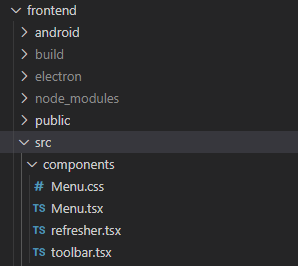
\includegraphics[width=0.7\linewidth]{images/implementation/frontend/frontend components.png}
    \caption{Componentes}
\end{figure}

\subsection{Páginas}
Como todo Frontend que se precie, debe tener distintas páginas, para así favorecer la correcta modularización de las funcionalidades.

Las páginas creadas son:
\begin{itemize}
    \item Home: página creada para ver de un vistazo todas las secciones de la aplicación.
    \item Crop: páginas creadas para hacer el CRUD sobre los cultivos.
    \item Events: páginas creadas para realizar la suscripción a los eventos complejos.
    \item FarmableLand: páginas creadas para hacer el CRUD sobre los terrenos.
    \item Irrigate: páginas creadas para hacer el CRUD sobre los riegos de los terrenos.
    \item Login: página creada para permitir el acceso correcto al sistema mediante la introducción correcta de las credenciales de usuario, formada por nombre de usuario y contraseña.
    \item Notifications: página creada para ver por orden de más cercano a más lejano en el tiempo todas las notificaciones al usuario.
    \item Phytosanitary: páginas creadas para hacer el CRUD sobre los fitosanitarios de los cultivos.
    \item Settings: página creada para ver y modificar los ajustes del sistema del usuario, tales como aspecto visual, idioma por defecto y acción por defecto en los eventos complejos.
\end{itemize}

\subsection{Servicios}
Para poder reutilizar código, hemos creado una capa de servicio formado principalmente por funciones útiles reutilizables para los principales comportamientos que se repiten a lo largo de la aplicación frontal, tales como obtener la información de sesión - ajustes o bien, acceder a los endpoints con el correspondiente token de sesión.

También se usan funciones para el sistema traducción, i18n \cite{i18n} \cite{i18n-react}, y para el sistema de push notificacions de Firebase \cite{firebase}.

\subsection{Routes}
Para poder usar características como ``ir hacia atrás'', hemos necesitado diseñar un sistema de routes usando como base el sistema que nos da React.

A partir de aquí, mediante URL, podemos acceder a cualquiera de las páginas en caso de usar la aplicación. En caso de la aplicación móvil, internamente también se usan las URLs, pero como se traslada a un sistema de vistas como en Android nativo, así que funciona igual pero sin acceso a escribir la URL que se desee.

\subsection{Environment}
Para establecer las variables de entorno como en el Backend, se necesita también crear archivos de la extensión .env.

En concreto, para React, reconoce dos tipos de perfiles. El de ejecución local con livereload y el de production donde se realiza el build. Así pues, en principio tenemos dos ficheros de variables de entorno, .env y .env.production.

Pero a parte, como nosotros construimos la aplicación móvil Android, pues hemos agregado un tercer fichero de variables de entorno llamado .env.android para probar ejecuciones en local. Cuando la aplicación se construya para un modo de producción como la plataforma Google Play Store, pues se usará el fichero .env.production.

Por último, antes de exponer las imágenes de los ficheros, queda aclarar que para que una tecnología como React lea las variables de entorno, dichas variables tienen que empezar por el prefijo REACT\_APP\_.

A continuación, exponemos los 3 ficheros de variables de entorno con sus respectivos valores en los Listados 6.13, 6.14 y 6.15.

\begin{lstlisting}[language=Java,caption={Fichero .env},captionpos=b]
REACT_APP_BACKEND_HOST=http://localhost:3000
REACT_APP_CHECK_SESSION_TIME=1000000
\end{lstlisting}

\begin{lstlisting}[language=Java,caption={Fichero .env.production},captionpos=b]
REACT_APP_BACKEND_HOST=https://backend-tfg.azurewebsites.net
REACT_APP_CHECK_SESSION_TIME=1000000
\end{lstlisting}

\begin{lstlisting}[language=Java,caption={Fichero .env.android},captionpos=b]
REACT_APP_BACKEND_HOST=http://10.0.2.2:3000
REACT_APP_CHECK_SESSION_TIME=1000000
\end{lstlisting}

\subsection{App}
Respecto a la creación de la instancia de la aplicación frontal, no tiene mucha variación respecto a una instancia de una aplicación frontal con React, salvo por la pecurialidad de nuestro proyecto donde además es imperativo instanciar a su vez un servicio de Firebase para las notificaciones.

\subsection{Android}
Para la aplicación Android, hemos usado el SDK de Ionic para poder construir con el comando \textbf{ionic capacitor build android}.
Pero, no es lo único que se necesita hacer para que la aplicación Android funcione, ya que, tiene su propia complejidad activar las Push Notifications y permitir el uso de internet en la aplicación Android.

A continuación, exponemos en los Listados 6.16 y 6.17 las líneas de código añadidas a los ficheros para que funcione todo correctamente.

\begin{lstlisting}[language=Java,caption={Fichero app/build.gradle},captionpos=b]
dependencies {
    implementation platform('com.google.firebase:firebase-bom:27.1.0')
    implementation 'com.google.firebase:firebase-analytics'
}
\end{lstlisting}

\begin{lstlisting}[language=XML,caption={Fichero AndroidManifest.xml},captionpos=b]
...
    <application
        android:allowBackup="true"
        android:icon="@mipmap/ic_launcher"
        android:label="@string/app_name"
        android:roundIcon="@mipmap/ic_launcher_round"
        android:supportsRtl="true"
        android:theme="@style/AppTheme"
        android:usesCleartextTraffic="true">
...
\end{lstlisting}

\subsection{Web}
Para la aplicación más usada como es la aplicación web del Frontend, solo tiene un particularidad con respecto al código base, y es que para que el servicio de notificaciones funcione, se necesita a parte un ``Service Worker'' para estar leyendo dichas notificaciones y mostrarlas en el frontal.

Para ejecutar la aplicación web, se puede usar el comando \textbf{ionic serve}.

\subsection{Desktop}
Por último, respecto a la aplicación frontal, existe la aplicación de escritorio. Esta aplicación se construye con el SDK de Ionic con el comando \textbf{ionic capacitor build electron}

\section{Sistema IoT}
Aquí expondremos las distintas partes que conforman el Sistema de IoT y como se relacionan entre sí.

\subsection{Emulator}
Como todo Sistema de IoT, tiene una parte de creación de eventos simples. En concreto, esto en nuestro proyecto se hace con la creación de un dispositivo virtual que simula dichos eventos simples.

\subsection{Stream Analytics}
Otra parte fundamental de un Sistema de IoT es la parte de los patrones.

Esto en nuestro proyecto se realiza con el servicio de Stream Analytics de Azure Cloud \cite{stream-analytics}, el cual tiene su propio lenguaje y características.

Como ejemplo de codificación del patrón de eventos simples, exponemos en el Listado 6.18 nuestro patrón o consulta para detectar el evento complejo ``Irrigate''.

\begin{lstlisting}[language=SQL,caption={ASASmartRural-Irrigate.asaql},captionpos=b]
SELECT
  sensorId AS sensorId,
  'Irrigate' AS EventFired,
  COUNT(*) AS count
INTO
  [CosmosDB]
FROM
  [IoTHub]
WHERE
  isAtDaytime = 1
  and
  isRaining = 0
  and
  airHumidity < 30
  and
  roomTemperature < 25
GROUP BY
  sensorId, TumblingWindow(minute, 1)
\end{lstlisting}

\subsection{Azure CosmosDB}
Por último, una parte que no puede faltar en un Sistema de IoT es la del postprocesamiento del evento complejo. Es decir, una vez que se ha disparado ese evento complejo, se debe realizar una acción.

Esta acción en un nuestro proyecto es almacenar dicho evento complejo en una base de datos NoSQL como es Azure CosmosDB. Esta base de datos actua como ``stage'' intermediario temporal, donde cada cierto periodo de tiempo, el Backend acudé a dicha base de datos, obtiene los eventos complejos lanzados y actúa en consecuencia.

Por supuesto, una vez que obtiene los datos, limpia la base de datos para que no surja repetición de los mismos.

A continuación, exponemos en la Figura 6.4 un ejemplo del tipo de datos que se almacena en la base de datos de Azure CosmosDB.

\begin{figure}[H]
    \centering
    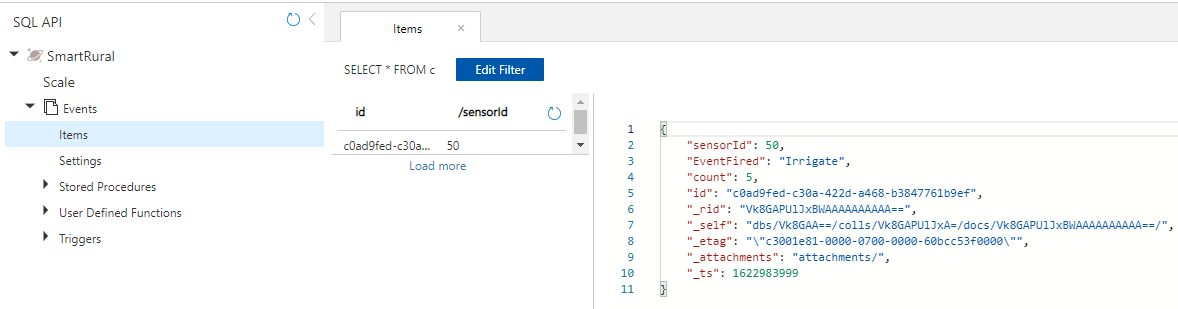
\includegraphics[width=1\linewidth]{images/implementation/iot/iot cosmosdb object.png}
    \caption{Azure CosmosDB Object}
\end{figure}